\documentclass{standalone}
\usepackage{tikz}
\usetikzlibrary{intersections}

\begin{document}
	
	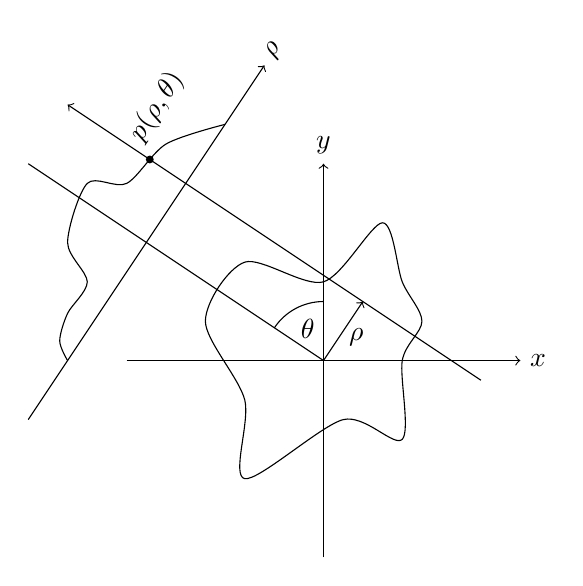
\begin{tikzpicture}[scale = 0.5]
		
		\draw[->] (-5, 0) -- (5, 0);
		\draw[->] (0, -5) -- (0, 5);
		\node[right] at (5, 0) {$x$};
		\node[above] at (0, 5) {$y$};
		
		\draw plot[smooth cycle] coordinates {(-3, 1) (-2, 2.5) (0, 2) (1.5, 3.5) (2, 2) (2.5, 1) (2, 0) (2, -2) (0.5, -1.5) (-2, -3) (-2, -1)};
		
		\draw[<-] (-1.5, 7.5) -- (-7.5, -1.5); %node[below right] {$\rho$};
		
		\draw[name path = ray, ->] (4, -0.5) -- (-6.5, 6.5);
		\draw (0, 0) -- (-7.5, 5);
		
		\draw (0, 1.5) arc (90 : 180 - atan(2 / 3) : 1.5);
		\node at (-0.4, 0.8) {$\theta$};
		
		\draw[->] (0, 0) -- (1, 1.5) node[pos = 0.4, right] {$\rho$};
		
		\draw[name path = radon] plot[smooth] coordinates {(-6.5, 0) (-6.7, 0.5) (-6.5, 1.2) (-6, 2) (-6.5, 3) (-6, 4.5) (-5, 4.5) (-4, 5.5) (-2.5, 6)};
		
		\fill[name intersections={of= radon and ray, total=\t}]
		\foreach \s in {1,...,\t}{(intersection-\s) circle[radius = 0.1] node[rotate= 90 - atan(2 / 3), above right] {$p(\rho, \theta)$}};
		
		\node[rotate= 90 - atan(2 / 3), right] at (-1.5, 7.5) {$\rho$};
		
	\end{tikzpicture}
	
\end{document}